

\begin{figure}
    \centering  % Centers the figure
    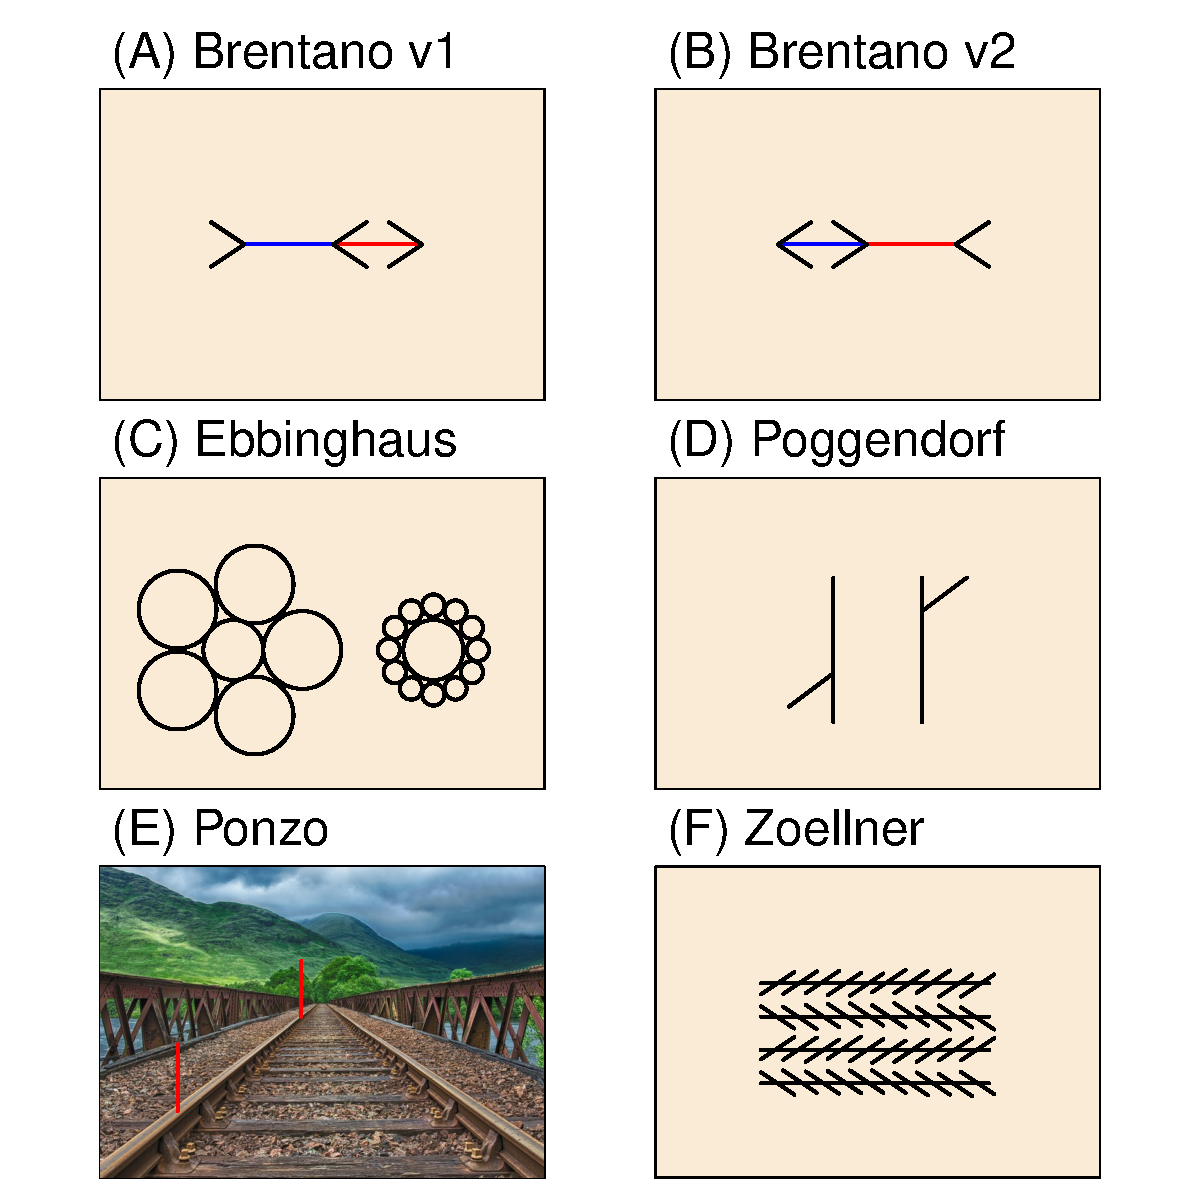
\includegraphics[width=6.5in, height=6.5in]{_figs/ill-tasks.pdf}
    \caption{{\bf Illusion Tasks:} A-B. Two versions of the Brentano Illusion were presented. Participants adjusted the center chevron so that the red and blue lines appeared equal in length. C. In the Ebbinghaus Illusion, participants adjusted the right inner circle in Version 1, while in Version 2, they adjusted the left inner circle. D. For the Poggendorf Illusion, participants adjusted the right lever vertically in Version 1. In Version 2, the illusion was flipped vertically, with the downward-facing right lever being adjusted on the right-hand side. E. In the Ponzo Illusion, participants adjusted the closer red line in Version 1 and the farther red line in Version 2. F. For the Zöllner Illusion, participants adjusted the horizontal lines to appear parallel. Version 1 is depicted in the figure and Version 2 was exactly the same but mirrored horizontally.}
    \label{fig:illPlots}
\end{figure}



\begin{figure}
    \centering  % Centers the figure
    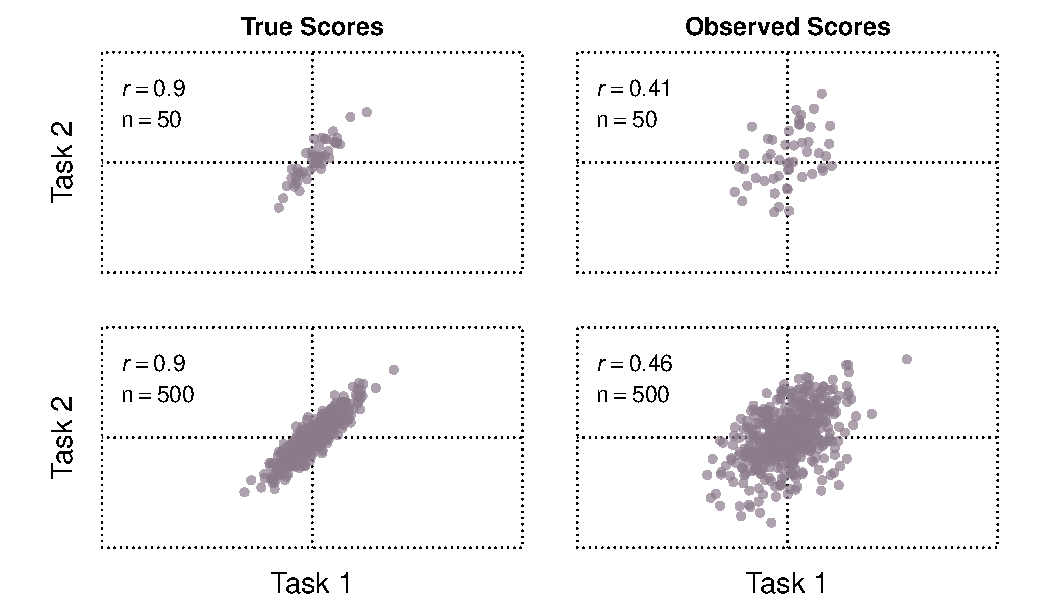
\includegraphics[width=7in, height=4in]{_figs/intro-plot.pdf}
    \caption{Trial noise leads to attenuation of correlations, with the left panel showing the true correlations between Task 1 and Task 2, and the right panel showing the observed correlations after introducing noise. Increasing the number of participants (n) does not mitigate this attenuation, as shown by the similar attenuation in correlation from true to observed scores regardless of the number of participants (n = 50 or n = 500).}
    \label{fig:introPlot}
\end{figure}





\begin{figure}
    \centering  % Centers the figure
    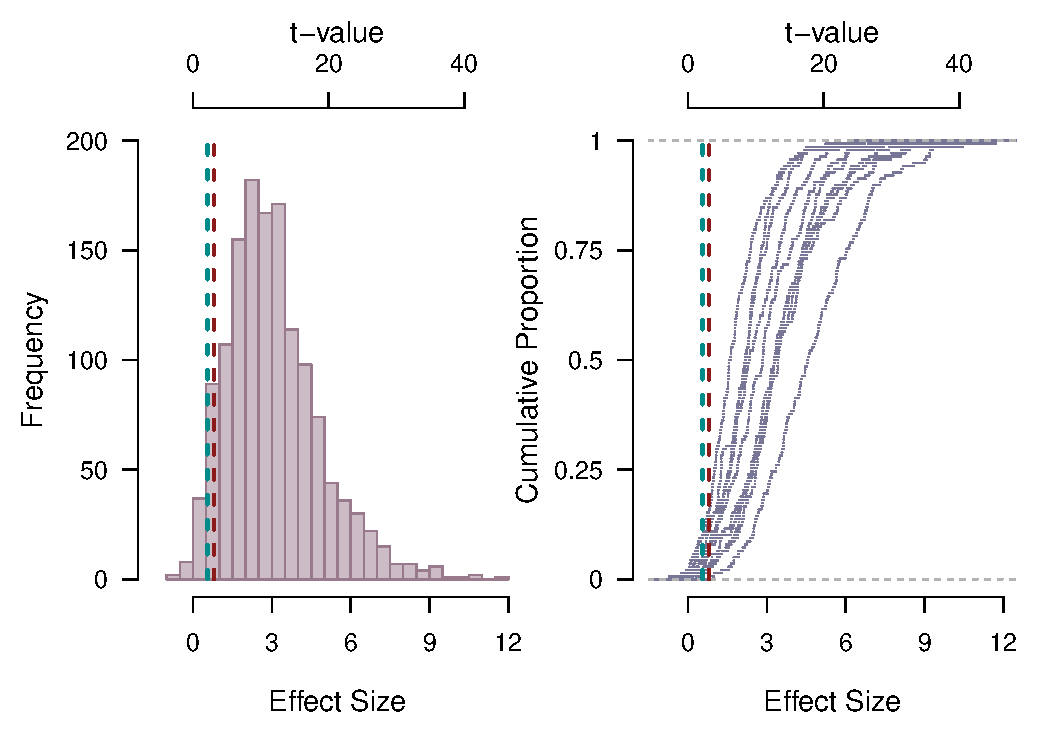
\includegraphics[width=6in, height=5in]{_figs/effect-plot.pdf}
    \caption{The size of illusions effects. The data from each participant in each task is treated as a separate experiment. Left: Histogram of all effect sizes shows large effects for almost all combinations of individuals and tasks.  Right: The same data plotted as an empirical-cumulative-distribution function reveals although there are large effects for all tasks, there are some differences across the tasks.}
    \label{fig:effectPlots}
\end{figure}

\begin{figure}
    \centering  % Centers the figure
    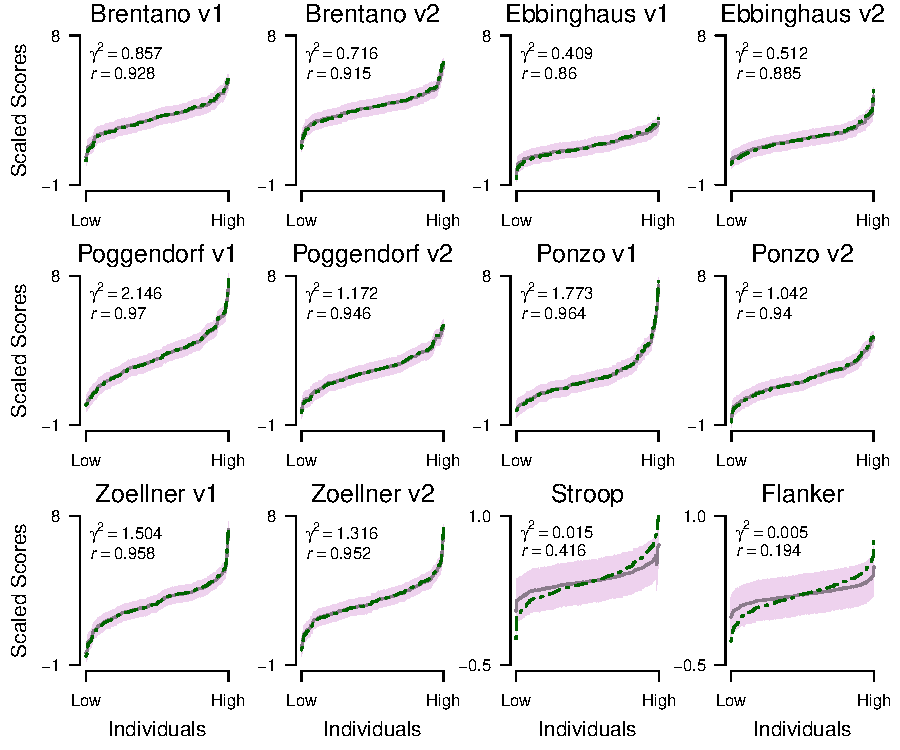
\includegraphics[width=6in, height=5in]{_figs/task_plots.pdf}
    \caption{Task plots for the 10 illusion tasks and two cognitive control tasks. Observed effects are shown as dashed lines, while the solid lines represent model-based estimates. The shaded area indicates the $95\%$ credible interval for the model-based effects. The task plots show individual effects ordered from smallest to largest. The illusion tasks demonstrate substantial variability in individual performance relative to noise, suggesting that studying individual differences is feasible even with a limited number of trials per task. In contrast, the two cognitive control tasks show only marginal individual differences when compared to trial noise.}
    \label{fig:taskPlots}
\end{figure}


\begin{figure}
    \centering  % Centers the figure
    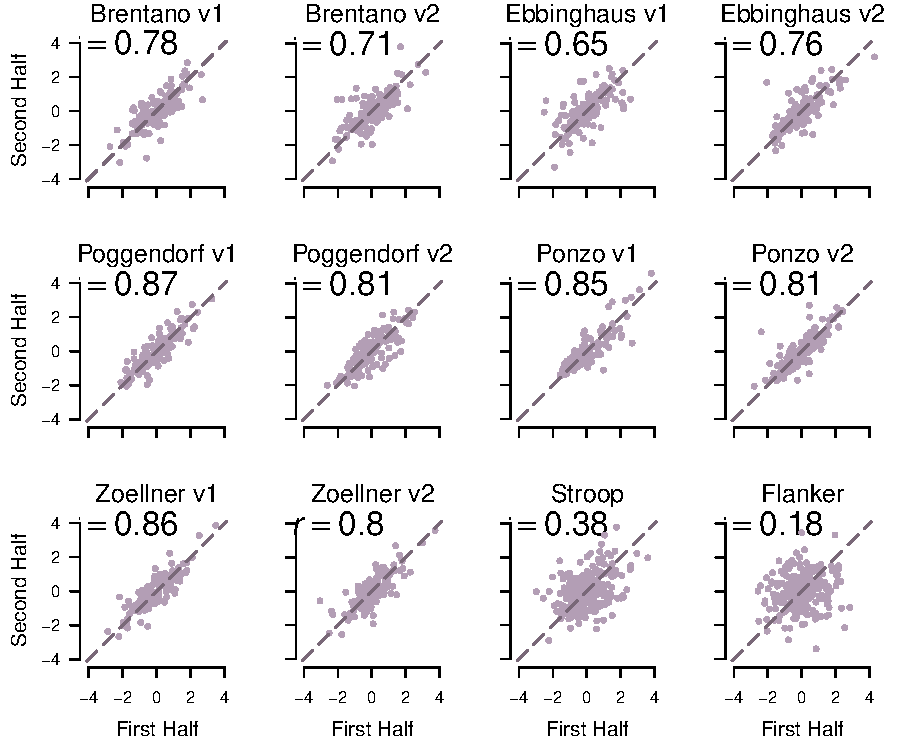
\includegraphics[width=6in, height=5in]{_figs/split-halves.pdf}
    \caption{Split-half reliabilities serve as check.  Even though the halves may differ systematically from learning and are comprised of 7 and 8 trials, respectively, the reliability is high.  Split-half reliability for cognitive control is less even though there are over 10X as many trials, and this result again highlights the lack of trial noise in illusion tasks compared to cognitive control tasks.}
    \label{fig:relPlots}
\end{figure}


\begin{figure}
    \centering  % Centers the figure
    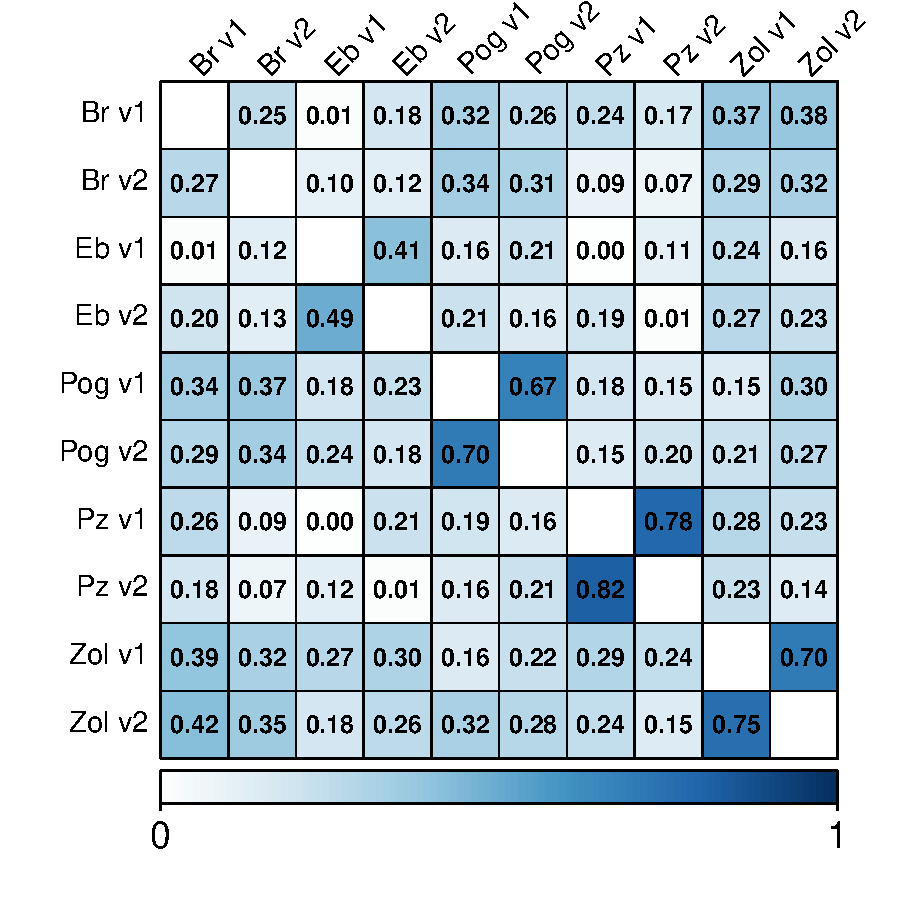
\includegraphics[width=6in, height=6in]{_figs/cor.pdf}
    \caption{Correlations across tasks.  The upper triangle shows sample correlations.  The lower triangle is model-estimated correlations from the hierarchical Wishart model.   Sample and model correlations are quite close reflecting a low degree of trial noise.  The defining features are large correlations between versions for the Poggendorf, Ponzo, and Zöllner Illusions, but more marginal correlations for Brentano and Ebbinghaus Illusions.}
    \label{fig:corPlot}
\end{figure}


\begin{figure}
    \centering  % Centers the figure
    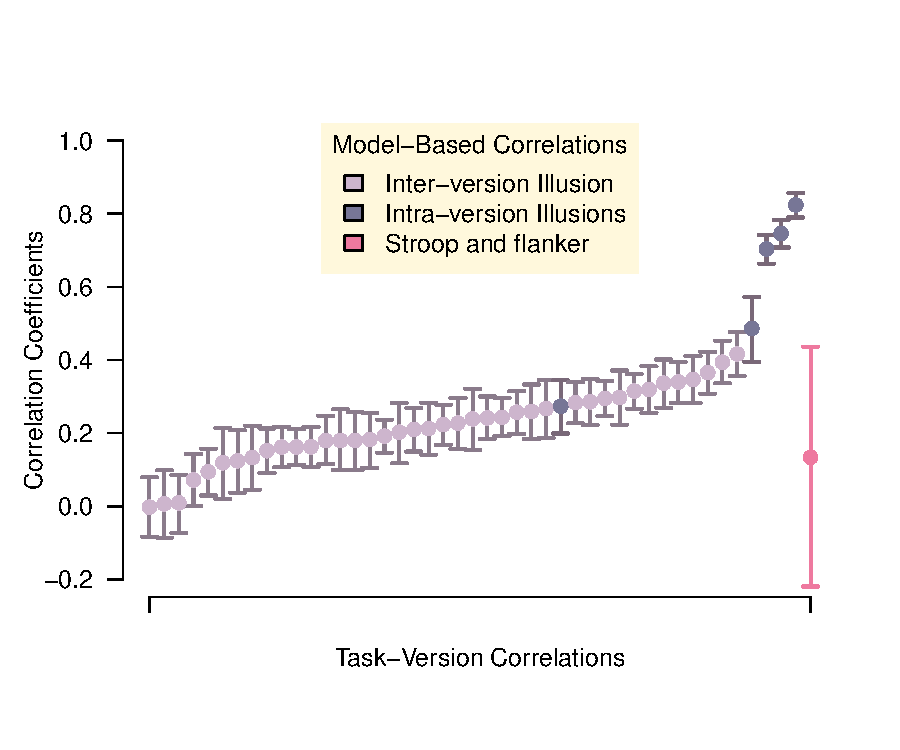
\includegraphics[width=6in, height=5in]{_figs/cor-CI.pdf}
    \caption{Uncertainties in correlations.  Shown are model correlations (lower triangle in Figure 5) along with 95\% credible intervals.  The three version correlations are well separated; the cross-task correlations center around .22 in value.}
    \label{fig:ciCorPlots}
\end{figure}


\begin{figure}
    \centering  % Centers the figure
    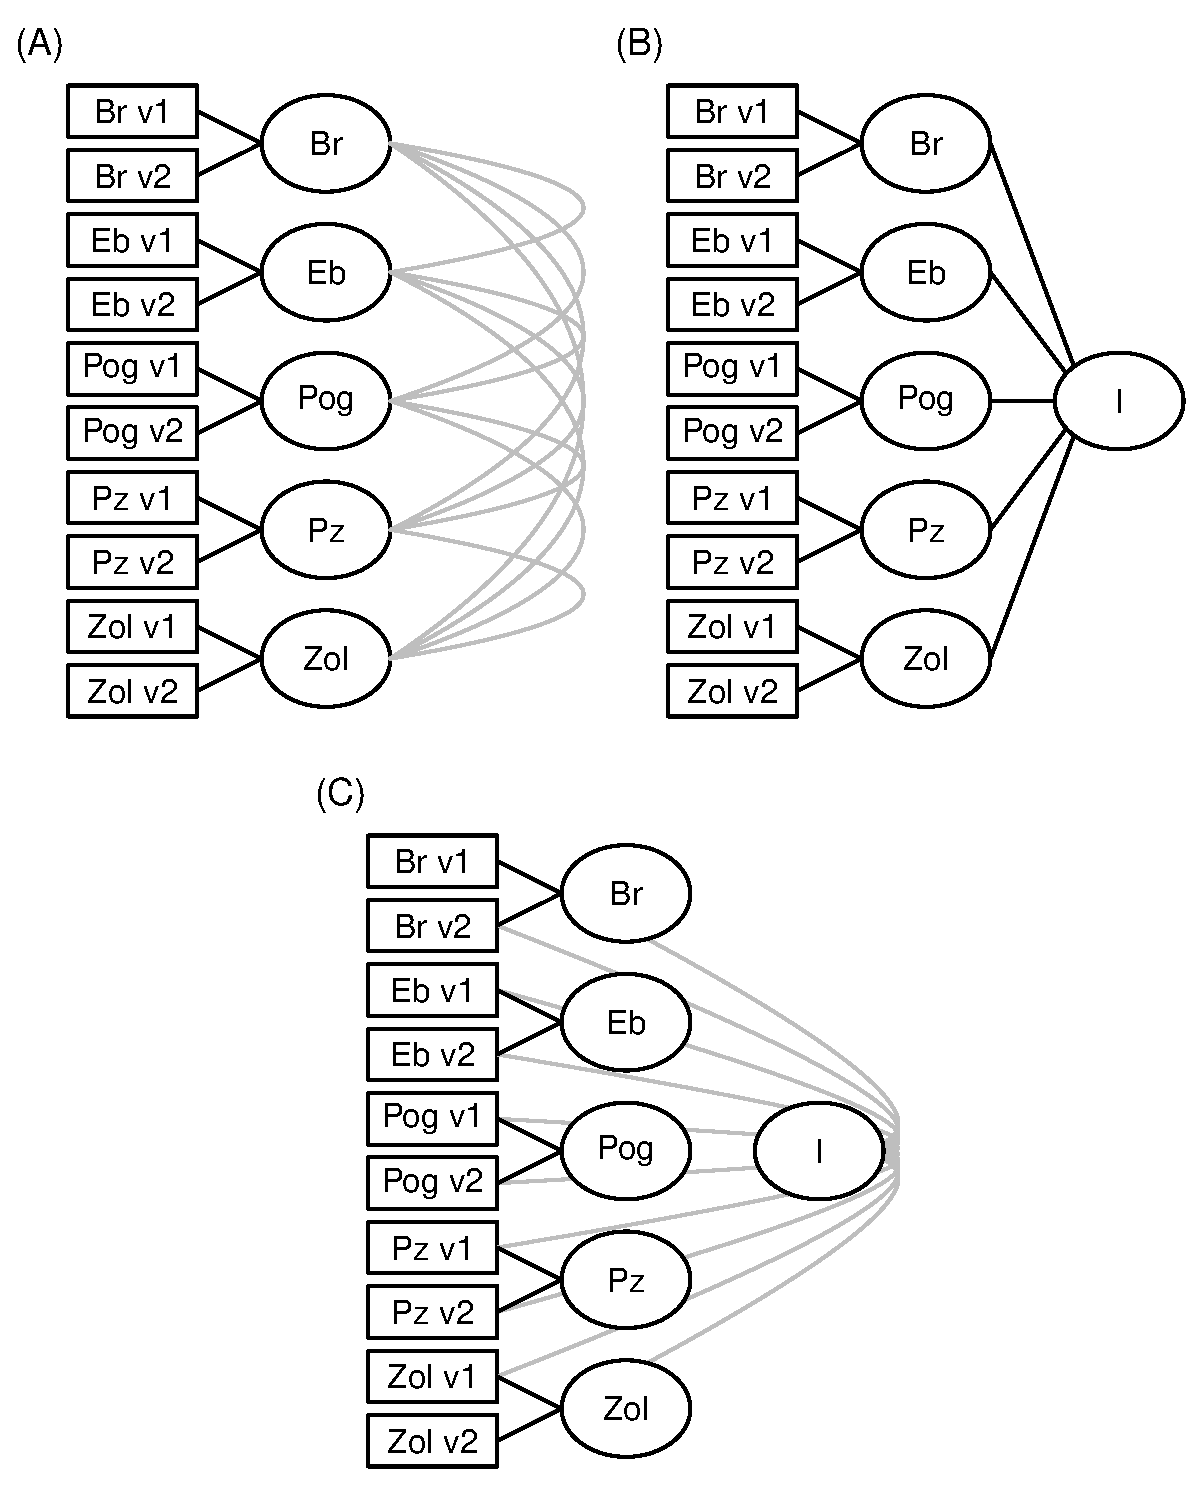
\includegraphics[width=6in, height=8in]{_figs/factor_cfa.pdf}
    \caption{Three confirmatory factor models did not yield interpretable results.}
    \label{fig:cfa}
\end{figure}


\begin{figure}
    \centering  % Centers the figure
    
\includegraphics[width=6in, height=3in]{_figs/efhbm.pdf}
    \caption{Summary of posterior estimates from the 7-factor hierarchical Bayesian model. (A) Task-wise projection onto the two general factors, where each arrow represents the average standardized loading of a task version on General Factor 1 (x-axis) and General Factor 2 (y-axis). (B) Posterior distributions of the proportion of total variance explained by each nuisance factor, which captures within-version idiosyncrasies for each illusion. (C) Posterior distributions of the proportion of total variance explained by the two general factors (black and gray), and the overall residual (unique) variance (red). All loadings and variance components are standardized to reflect proportions in the correlation metric.}
    \label{fig:efhbm}
\end{figure}